%%%%%%%%%%%%%%%%%%%%%%%%%%%%%%%%%%%%%%%%%%%%%%%%%%%%%%%%%%%%
% Document settings
\documentclass{ACGSeminar}

\usepackage{tikz}
\usepackage{svg}
\usepackage{mathtools}
\usepackage{tikz-3dplot}
\usepackage{pst-all}
\usepackage{pstricks}
\usepackage{pstricks-add}
\usepackage{graphicx}
\usepackage{pspicture}
\usepackage{scrextend}
\usepackage{pgfplots}
\usepgfplotslibrary{polar}
\usetikzlibrary{pgfplots.polar}
\usepackage{forest}

\bibliography{references}

%%%%%%%%%%%%%%%%%%%%%%%%%%%%%
% Hyphenations here
%%%%%%%%%%%%%%%%%%%%%%%%%%%%%
\hyphenation{}

%%%%%%%%%%%%%%%%%%%%%%%%%%%%%
% Title, Author, etc.

\begin{document}

\title{Efficient Ray Tracing Techniques}

\author{Dario Seyb}

\maketitle

%%%%%%%%%%%%%%%%%%%%%%%%%%%%%%%%%%%%%%%%%%%%%%%%%%%%%%%%%%%%
% Abstract

\begin{abstract}
Ray Tracing is next to rasterization the most widely used technique to generate discrete 2D images from continuous 3D scenes. Until recently ray tracing was too resource intensive to produce images in realtime, but advances in algorithms and hardware capabilities, most notably the introduction of GPGPU (General Purpose Graphics Processing Units), made near-realtime ray tracing feasible. In this report we will present some of the techniques which are used to achieve this.
\end{abstract}

\keywords{Ray Tracing, Acceleration Structures, Realtime Rendering, GPGPU}
\tableofcontents

%%%%%%%%%%%%%%%%%%%%%%%%%%%%%%%%%%%%%%%%%%%%%%%%%%%%%%%%%%%%
% Introduction

\section{Introduction} \label{introduction}
\subsection{Motivation}
Ray tracing is a technique used to synthesize photo-realistic images from a 3D scene description. This is useful in many applications, from architectural visualization, games and movies to medical imaging. While the rendered images are of very high quality, the time needed to produce even one frame of animation is usually in the minutes or hours. Big animation studios like Disney or Pixar can afford super computers to render their movies\footnote{http://www.engadget.com/2014/10/18/disney-big-hero-6/}, but this is not feasible for smaller companies or individuals. Luckily, with the advent of general purpose computation on consumer grade GPUs most people have a small super computer sitting in their PCs. The new NVIDIA GTX 1080 for example can do about 9 TFLOP/s \footnote{https://twitter.com/nvidia/status/728771223522410496}, as many as the fastest super computer in the world in 2001\footnote{http://www.top500.org/}.

Real time ray tracing is appealing, especially in the context of creative work, because it allows artists to preview changes to the scene immediately. Where you previously had to change the position or color of a light and wait until the next day to review the difference you can now tweak scenes interactively. This leads to a lower turn around time on changes in visuals and thus higher quality results.

\begin{figure}[htb!]
  \begin{centering}
    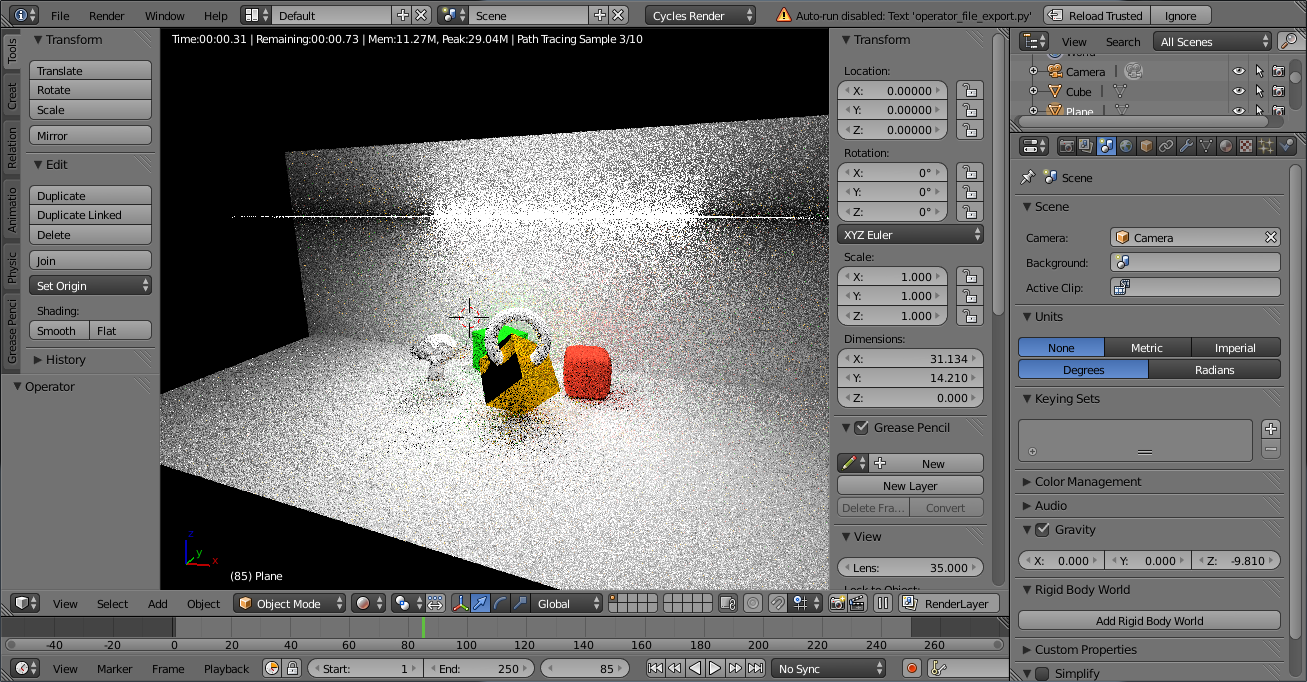
\includegraphics[width=12cm,natwidth=1307,natheight=682]{figures/blender_preview.png}\par
  \end{centering}
  \caption{Interactive ray traced scene view in Blender (blender.org).}
  \label{fig:blender_preview}
\end{figure}

In this report I will:
\begin{itemize}
\item Describe a state of the art ray tracing algorithm. (Section \ref{path-tracing})
\item Introduce techniques to reduce the time spent on ray-scene intersections. (Section \ref{acceleration})
\item Explain how to use the fact that the algorithm is running at interactive frame rates to improve image quality. (Section \ref{noise})
\item Give an overview over how to parallelize the construction of acceleration structures (Section \ref{gpu-adapting}) 
\item Present an implementation which incorporates the ideas described in this report. (Section \ref{results})
\end{itemize}


\subsection{A short history of ray tracing}
The technique of tracing rays through a scene consisting of primitives and media has been known to the computational physics community for a long time. There it is mostly used to simulate the propagation of waves (e.g. shock waves of an earthquake) through a heterogeneous medium (e.g. the interior of the earth). \cite{GJI:GJI93}

It was first described in relation to computer graphics by Arthur Appel in 1968. At the time the common method to visualize three dimensional scenes was to synthesize two dimensional line and point drawings. Appel recognized the importance of shading and shadow casting in conveying shape and spatial relations. In his paper "Some techniques for shading machine renderings of solids" he proposes a method to realize this shading by casting rays originating from the viewers' position through each pixel on the viewing plane and calculating the first point of intersection with the scene. To determine shading he casts a second ray from this intersection point to the light source. Appel's technique was very compute intensive for its time, but already illustrated the power of ray tracing to generate realistic images using a relatively simple algorithm. \cite{Appel68}

\begin{figure}[htb!]
  \begin{centering}
    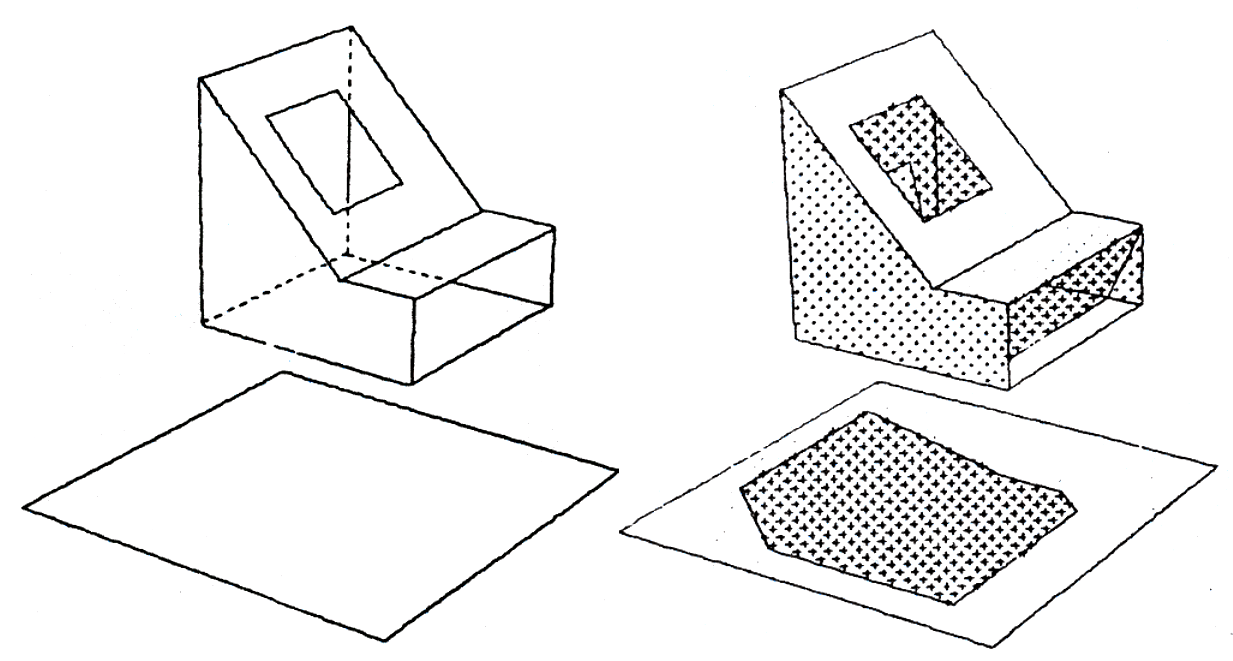
\includegraphics[width=12cm,natwidth=1233,natheight=661]{figures/Appel_Shading.png}\par
  \end{centering}
  \caption{Left: Unshaded Line/Point Drawing, Right: Drawing augmented with the technique introduced in \cite{Appel68}}
  \label{fig:appel_tracing}
\end{figure}

The next major contribution to ray tracing came from Turner Whitted of Bell Laboratories in 1980. In his landmark paper "An Improved Illumination Model for Shaded Display" \cite{Whitted:1980} he describes the algorithm that would become known as Recursive, or Whitted, Ray Tracing. So far ray tracing was only used to compute local illumination at the first point of intersection and the only secondary rays that were cast were shadow rays. This produced a fairly good approximation for diffuse surfaces, but was lacking in scenes with very reflective objects. Whitted took the concept of casting secondary rays and extended it to reflections and refractions. For each intersection point he proposed to not only compute a shadow ray in the direction of each light source, but also recursively compute the color of incoming reflected and refracted light. This technique produced impressive looking results, but Whitted himself acknowledged that it did not provide a solution to global illumination since objects could not act as light sources themselves and diffuse interreflections where not accounted for.

\begin{figure}[htb!]
  \begin{centering}
    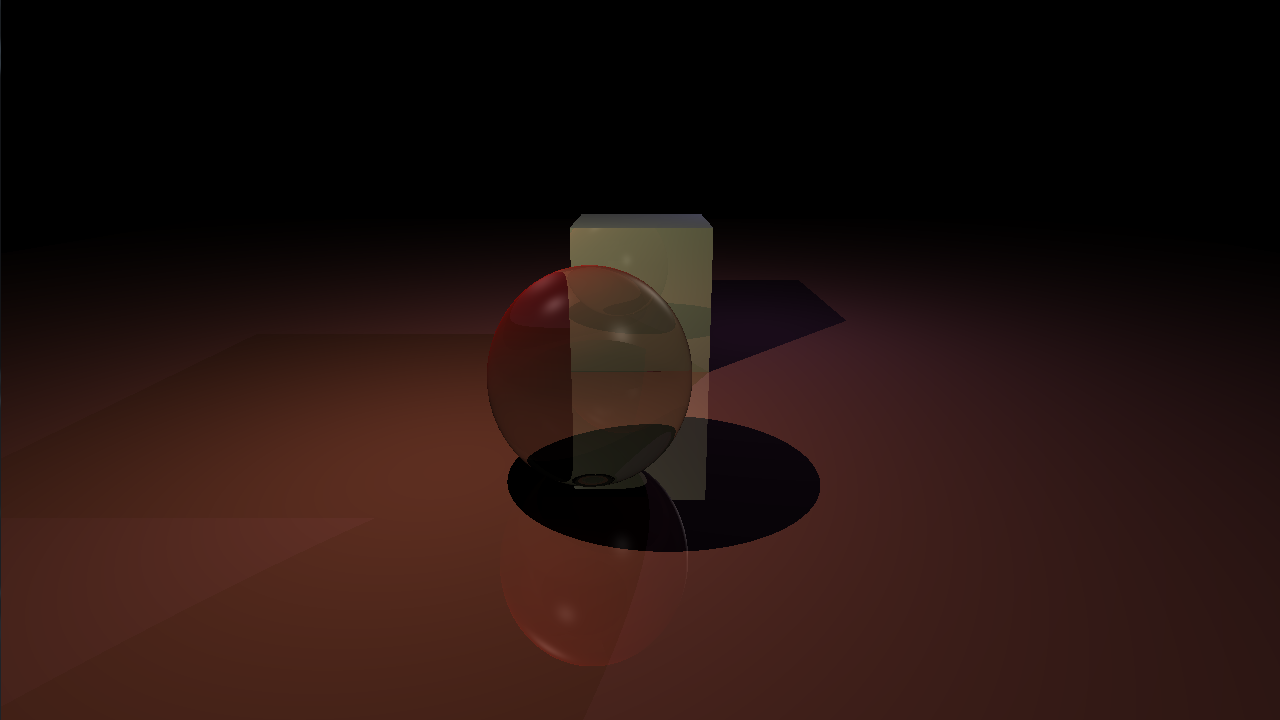
\includegraphics[width=12cm,natwidth=1280,natheight=720]{figures/whitted_raytracing.png}\par
  \end{centering}
  \caption{Whitted Ray Tracing implemented in the offline renderer "Zaphod" \cite{Zaphod}.}
  \label{fig:whitted-example}
\end{figure}


Over the next years many different approaches to solve this issue where proposed and in 1986 James T. Kajiya published a paper titled "The Rendering Equation"  \cite{Kajiya:1986} in which he presents an equation to describe the propagation of light in a scene. It is general enough to describe all optical phenomena we care about in computer graphics and this made it possible to classify rendering algorithms by how well they approximate a solution to the rendering equation.

\begin{equation} \label{eq:rendering-equation}
I(x,x')= \overbrace{g(x,x')}^{\mathclap{\text{Geometry Term}}}
         [
         \underbrace{\epsilon(x,x')}_{\mathclap{\text{Emission}}}
         + \underbrace{
         \int_{S}{\overbrace{p(x,x',x'')}^{\mathclap{\text{BRDF}}}
                  \overbrace{I(x',x'') }^{\mathclap{\text{Incoming light}}} dx''}
         }_{\mathclap{\text{Light reflected at $x'$ in direction $\overrightarrow{x'x}$}}} ]
\end{equation}
It describes the light transport between two points $x$ and $x'$ as a combination of emitted and reflected light at $x'$. The geometry term describes the amount of light that actually arrives at $x$ (e.g. $g(x,x') = 0$ if there is an object between the two points). To compute the reflected light we need to integrate over all directions in the hemisphere $S$ above point $x'$. 
The main difference between rendering algorithms is how they approach the evaluation of this integral. It cannot be evaluated analytically for scenes which are even remotely interesting, but the formulation of the rendering problem as an integral equation allows us to employ methods from calculus to devise new algorithms.

%%%%%%%%%%%%%%%%%%%%%%%%%%%%%%%%%%%%%%%%%%%%%%%%%%%%%%%%%%%%
% Second Section
\section{Overview over the path tracing algorithm} \label{path-tracing}
Path tracing is an algorithm which solves the integral in \eqref{eq:rendering-equation} by randomly sampling it. This process is also called "Monte Carlo integration". \cite{veach1997robust} Each sample is represented by a list of points $(x_0, ..., x_n), x_i \in \R^3$ which form a path through space. This is similar to Whitted Ray Tracing, except that the points are randomly chosen instead of being predetermined by the reflection and refraction directions. The final value of a path sample is calculated using Equation \eqref{eq:rendering-equation}, recursively evaluating it for $x_0$ to $x_n$. 

\begin{figure}[htb!]
  \centering
  % Sketch output, version 0.3 (build 7, Fri Feb 24 21:22:17 2012)
% Output language: PSTricks,LaTeX
\begin{pspicture}(-1,-1)(2,2)
% If your PSTricks is earlier than Version 1.20, it will fail here.
% Use sketch -V option for backward compatibility.
\psset{linejoin=1}
\psline(-1,-1)(.333,.333)
\pspolygon[fillstyle=solid,fillcolor=white](0,0)(1,0)(0,1)
\psline(.333,.333)(2,2)
\end{pspicture}% End sketch output

  \caption{A light path through a scene.}
  \label{fig:light-path}
\end{figure}

In classical path tracing paths start at a point on the image plane. A first intersection point in the scene is calculated. At this point a scattering event is simulated. This is done by randomly choosing a new direction with a distribution which depends on the material of the hit object. The next intersection is calculated based on the chosen direction.

\begin{figure}[htb!]
  \begin{centering}
    \tdplotsetmaincoords{0}{0}
    \begin{tikzpicture}[tdplot_main_coords]
      \draw[thick,-] (-4,0) -- (4,0) node[anchor=north east]{Surface};
      \draw[thick,->] (0,0) -- (0,2.5) node[anchor=north west]{$\vec{n}$};
      \draw[thick,<-] (0,0) -- (-3.5,3.0)
                      node[anchor=south east]{$\overrightarrow{x_{i-1}x_i}$};
      \tdplotdefinepoints(0,0,0)(0,2,0)(-3.5,3.0,0);
      \tdplotdrawpolytopearc[thin,<->]{1.25}{anchor=south}{$\omega_0$};
      \draw[thick,dashed,->] (0,0) -- (3.5,1.5)
                             node[anchor=south west]{$\overrightarrow{x_ix_{i+1}}$};
      \tdplotdefinepoints(0,0,0)(0,2,0)(3.5,1.5,0);
      \tdplotdrawpolytopearc[thin,<->]{1.5}{anchor=south}{$\omega_1$};
      \draw[thin, densely dotted, <-] (0,0) -- (1, 0) arc (0:180:1cm) -- cycle;
      \draw (1,0) node[below]{$S$};
      \draw (0,0) node[below]{$x_i$};
    \end{tikzpicture}\par
  \end{centering}
  \caption{Geometry of a single scattering event.}
  \label{fig:scattering-event}
\end{figure}

A path is terminated when (1) it reaches a light source (2) the maximum path length is reached (3) no intersection is found.
The reason why paths start at the camera is that a path which starts at some point on the surface of a light source is very unlikely to hit the image plane. More sophisticated methods like Bidirectional Path Tracing start rays at both ends and try to connect them, but those are outside the scope of this report.

\section{Acceleration Structures} \label{acceleration}
Intersection tests are by far the most expensive part of any ray tracing algorithm. \cite[7]{Whitted:1980} This is true even for simple scenes, but becomes a major performance issue in large scenes. Ideally we would like the performance of a ray tracer to be independent from scene complexity, but this is no possible when using a classical polygon based scene representation.
Rasterization renderers usually perform a culling operation to exclude objects which are not in view of the camera from being rendered. Unfortunately that is not helpful for path tracing since secondary rays can require intersection tests with off-screen objects.
The naive implementation of a ray cast performs an intersection test with every primitive in the scene. Hence it scales linearly with the number of primitives. Acceleration structures which partition either objects or space allow us to do better. They generally reduce the time complexity of a ray cast from $O(n)$ to $O(\log n)$ in the number of primitives. In the following I will discuss various commonly used acceleration structures. The main trade off is usually construction time versus ray tracing performance. Generally, structures which offer better ray tracing performance take longer to set up and are mostly suited for static scenes, while structures which trade in some ray tracing performance for shorter set up times are better suited for real time applications and dynamic scenes. \cite{Karras:2012:MPC:2383795.2383801}

\subsection{BSP and KD-Trees}
The first class of acceleration structures are space partitioning trees. They split the scene into smaller and smaller sub-spaces which are wholly contained in their parent space. It is also recorded which objects belong to which sub-space. Once the tree is constructed a ray-scene intersection algorithm can start at the root node and only traverse into sub trees if the ray intersects with their parent node. Actual ray-primitive intersection tests are only necessary once a leaf node is reached. If the tree is well constructed this reduces the number of intersection tests dramatically.
BSP Trees split space recursively along splitting planes. In the general BSP tree the orientation of the splitting plane can be chosen freely. KD-trees are a subclass of BSP trees where the splitting planes are axis aligned. This makes kd-trees substantially easier to construct since there are less degrees of freedom for the splitting planes. The drawback is that there are situations where a BSP tree might be faster to traverse than a kd-tree.
Algorithms which construct an optimal kd-tree are NP complete. [TODO:FIND REFERENCE] In practice heuristics are used, the most successful one being the surface area heuristic. \cite{MacDonald1990}

\begin{figure}[htb!]
  \centering
  %LaTeX with PSTricks extensions
%%Creator: 0.48.3.1
%%Please note this file requires PSTricks extensions
\psset{xunit=.5pt,yunit=.5pt,runit=.5pt}
\begin{pspicture}(336.18011475,183.29096985)
{
\newrgbcolor{curcolor}{0 0 0}
\pscustom[linewidth=1,linecolor=curcolor]
{
\newpath
\moveto(59.599,153.03811185)
\lineto(124.248764,179.30207785)
\lineto(181.322384,109.60155185)
\lineto(114.147234,103.03556085)
\lineto(82.327434,62.62946185)
\closepath
}
}
{
\newrgbcolor{curcolor}{0 0 0}
\pscustom[linewidth=1,linecolor=curcolor]
{
\newpath
\moveto(247.48737,104.04571185)
\lineto(150.00765,65.65991985)
\lineto(143.94674,28.28426985)
\lineto(236.3757,16.16243985)
\lineto(285.87317,53.53808985)
\closepath
}
}
{
\newrgbcolor{curcolor}{1 0 0}
\pscustom[linestyle=none,fillstyle=solid,fillcolor=curcolor]
{
\newpath
\moveto(17.67767,8.58629985)
\lineto(327.28942,178.29192435)
}
}
{
\newrgbcolor{curcolor}{0 1 0}
\pscustom[linewidth=1,linecolor=curcolor]
{
\newpath
\moveto(17.67767,8.58629985)
\lineto(327.28942,178.29192435)
}
}
{
\newrgbcolor{curcolor}{0.56078434 0.56078434 0.56078434}
\pscustom[linewidth=1,linecolor=curcolor,linestyle=dashed,dash=1 1]
{
\newpath
\moveto(177.78685,177.28177185)
\lineto(177.78685,6.56598985)
}
}
{
\newrgbcolor{curcolor}{0.48627451 0.48627451 0.48627451}
\pscustom[linewidth=1,linecolor=curcolor,linestyle=dashed,dash=1 1]
{
\newpath
\moveto(329.309724,94.44926185)
\lineto(8.08122,94.44926185)
}
}
\end{pspicture}

  \caption{A scene which can be split using a BSP tree, but not a kd-tree.}
  \label{fig:bsp-trees}
\end{figure}

Efficient traversal is achieved by always traversing the child node which lies closer to the ray origin first.

\subsection{Bounding Volume Hierarchies}
On a first glance BVHs look very similar to BSP trees. The difference is that BVHs group objects together while BSP trees split space recursively. A common choice for bounding volumes are spheres and axis aligned bounding boxes because they are cheap to construct, require little additional memory and their ray intersection tests are fast. More complex bounding volumes like object oriented bounding boxes, discrete oriented polytopes or convex hulls are attractive because they can provide a tighter fit, but this is usually far outweighed by the added complexity and storage requirements.
Again, algorithms which find optimal BVHs are NP complete and heuristics have to be used.

\section{Reducing Noise} \label{noise}
For classical path tracing to converge to a stable solution we need to sample thousands of paths for each pixel. Since sampling a path requires intersection tests which are already the bottleneck of the pipeline this is not something we can afford under the constraints of real time rendering. The lack of samples results in a high variance between pixels which is expressed as noise. While uniform noise is one of the more pleasant artefacts in computer graphics it still impacts the perceived quality of rendered images. [TODO: FIND STUDY]
In the following I will describe two approaches to reduce variance and improve image quality without sampling more paths.
\begin{itemize}
\item \textbf{Reducing the variance} of the sampled paths by carefully choosing the sampled distribution in our Monte Carlo integrator.
\item \textbf{Reusing samples} from previous frames and thus reducing variance by having a larger number of samples for each pixel.
\end{itemize}

\subsection{Importance Sampling}
In his thesis Eric Veach presents a number of ways to reduce variance in Monte Carlo algorithms. \cite[45--70]{veach1997robust} I will focus on importance sampling \cite[47--48]{veach1997robust}, because it is easy to integrate into existing algorithms. Other techniques such as Bidirectional Path Tracing or Metropolis Light Transport produce better results, but are more complicated to implement correctly, especially on the GPU.

The idea of importance sampling is to concentrate our efforts on parts of the integral in Equation \eqref{eq:rendering-equation} which have a large value. That is, we would rather sample paths which contribute a lot to the image than paths which barely do. To achieve this we choose a function $g$ that is as similar as possible to the function $f$ we want to evaluate and which can be sampled efficiently. A common technique is to approximate or disregard factors in f until we arrive at a function which can be integrated analytically. In the case of path tracing $f = p(x,x',x'')I(x',x'')$ where $p$ is a BRDF. The factor of $f$ that makes it especially hard to integrate analytically or approximate is $I(x',x'')$ since $I$ is defined recursively (see Equation \eqref{eq:rendering-equation}). If we disregard $I(x',x'')$ we are left with $p(x,x',x'')$ which is much easier to reason about. While not all BRDFs can be solved analytically \cite{Montes2012} they are usually designed to be sampled with a given probability distribution, which gives us the approximation $g$ we were looking for. 

\begin{figure}[htb!]
  \begin{centering}
  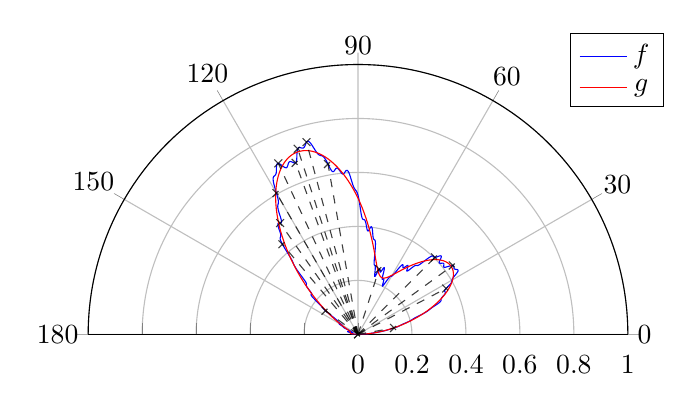
\begin{tikzpicture}
   \begin{polaraxis}[xmin=0,xmax=180,ymax=1,
    ytick align=outside,
    yticklabel style={
        anchor=north,
        yshift=-2*\pgfkeysvalueof{/pgfplots/major tick length}
    }]
	\addplot+[mark=f,domain=0:180,samples=600] 
		{cos(x-90)*(sin(2*x)*cos(2*x) + cos(0.3*x + 1) - sin(30*x)*0.05 + cos(100*x)*0.02)/1.75 }; 
    \addplot+[mark=g,domain=0:180,samples=600] 
		{cos(x-90)*(sin(2*x)*cos(2*x) + cos(0.3*x + 1))/1.75 };
    \addplot+[dashed, polar comb,domain=0:180, samples=6,black,opacity=0.75,mark=x]
	    {cos(x-90)*(sin(2*x)*cos(2*x) + cos(0.3*x + 1) - sin(30*x)*0.05 + cos(100*x)*0.02)/1.75  };
	\addplot+[dashed, polar comb,domain=10:45, samples=3,black,opacity=0.75,mark=x]
	    {cos(x-90)*(sin(2*x)*cos(2*x) + cos(0.3*x + 1) - sin(30*x)*0.05 + cos(100*x)*0.02)/1.75  };
	\addplot+[dashed, polar comb,domain=100:130, samples=4,black,opacity=0.75,mark=x]
	    {cos(x-90)*(sin(2*x)*cos(2*x) + cos(0.3*x + 1) - sin(30*x)*0.05 + cos(100*x)*0.02 )/1.75 };
	\addplot+[dashed, polar comb,domain=105:125, samples=3,black,opacity=0.75,mark=x]
	    {cos(x-90)*(sin(2*x)*cos(2*x) + cos(0.3*x + 1) - sin(30*x)*0.05 + cos(100*x)*0.02 )/1.75 };
	\legend{$f$, $g$}
	\end{polaraxis}
  \end{tikzpicture}\par
  \end{centering}
  \caption{Approximating a complicated function $f$ by a simpler function $g$ and sampling $f$ based on the probability distribution of $g$. Note how we are more likely to sample the $f$ in directions where it has a large value.\protect\footnotemark}
  \label{fig:importance-sampling}
\end{figure}
\footnotetext{$f$ and $g$ are chosen for illustration purposes only and are not supposed to represent an actual BRDF.}

The most basic example of importance sampling is using the fact that all BRDFs must account for Lambert's cosine law. Just by using the distribution in Figure \ref{fig:cosine-dist} we can reduce the variance dramatically since we avoid sampling rays which are almost parallel to the surface and thus don't contribute much to its illumination. [TODO: REFERENCE]

To keep the expected value of the Monte Carlo integration the same we need to account for the fact that we are no longer sampling $f$ uniformly. This is done by simply dividing the sampled value by the probability of choosing that value since

\begin{equation}
E[\frac{1}{N} \sum_{i=1}^{N} f(X_i)], X \sim U = E[\frac{1}{N} \sum_{i=1}^{N} \frac{f(X_i)}{p(X_i)}], X \sim p
\end{equation}

There is a lot of value in finding a good approximation to a BRDF since sampling even relatively complex approximations is very cheap compared intersection tests. Better importance sampling directly correlates with less variance and thus reduces the number of needed path samples per pixel dramatically.

\begin{figure}[htb!]
  \begin{centering}
  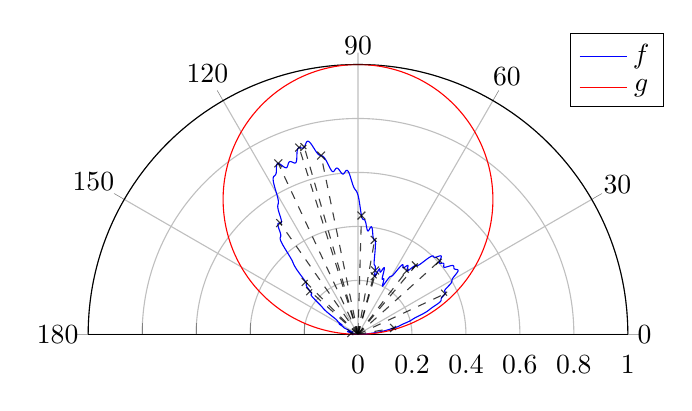
\begin{tikzpicture}
   \begin{polaraxis}[xmin=0,xmax=180,ymax=1,
    ytick align=outside,
    yticklabel style={
        anchor=north,
        yshift=-2*\pgfkeysvalueof{/pgfplots/major tick length}
    }]
    \addplot+[mark=f,domain=0:180,samples=600] 
		{cos(x-90)*(sin(2*x)*cos(2*x) + cos(0.3*x + 1) - sin(30*x)*0.05 + cos(100*x)*0.02)/1.75 }; 
	\addplot+[mark=f,domain=0:180,samples=600] 
		{ cos(x-90)};
		
    \addplot+[dashed, polar comb,domain=10:170, samples=6,black,opacity=0.75,mark=x]
	    {cos(x-90)*(sin(2*x)*cos(2*x) + cos(0.3*x + 1) - sin(30*x)*0.05 + cos(100*x)*0.02)/1.75  };
	\addplot+[dashed, polar comb,domain=25:135, samples=5,black,opacity=0.75,mark=x]
	    {cos(x-90)*(sin(2*x)*cos(2*x) + cos(0.3*x + 1) - sin(30*x)*0.05 + cos(100*x)*0.02)/1.75  };
	\addplot+[dashed, polar comb,domain=50:125, samples=2,black,opacity=0.75,mark=x]
	    {cos(x-90)*(sin(2*x)*cos(2*x) + cos(0.3*x + 1) - sin(30*x)*0.05 + cos(100*x)*0.02 )/1.75 };
	\addplot+[dashed, polar comb,domain=75:115, samples=4,black,opacity=0.75,mark=x]
	    {cos(x-90)*(sin(2*x)*cos(2*x) + cos(0.3*x + 1) - sin(30*x)*0.05 + cos(100*x)*0.02 )/1.75 };
    \legend{$f$, $g$}
	\end{polaraxis}
  \end{tikzpicture}\par
  \end{centering}
  \caption{Sampling a distribution $g$ which only accounts for Lambert's cosine law}
  \label{fig:cosine-dist}
\end{figure}

\begin{figure}[htb!]

  \centering
  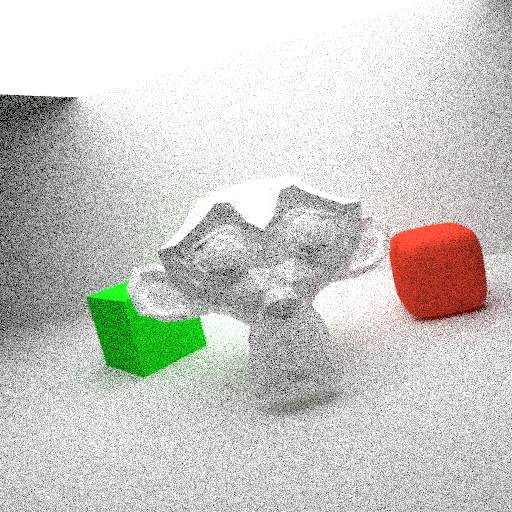
\includegraphics[width=5cm,natwidth=512,natheight=512]{figures/50_spp_cosine_weighted.png}
  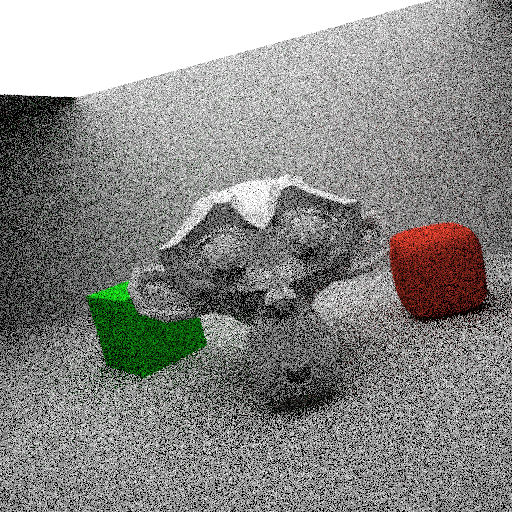
\includegraphics[width=5cm,natwidth=512,natheight=512]{figures/50_spp_uniform.png}
  \caption{Left: Cosine Weighted Sampling, Right: Uniform Sampling TODO: GET CORRECT RENDERS OF BOTH CASES}
  \label{fig:rendering-cos-weighted}
\end{figure}

\subsection{Temporal Supersampling}
Ray tracing research has mostly focused on the previous area for variance reduction since the common use case is rendering still images.
In real time rendering we are generating an output image 30-60 times per second. Usually the changes between frames are small (i.e. we can assume temporal coherency). Classical rasterization based rendering pipelines re-render the whole image every frame and disregard previous results completely. This has established itself since samples per pixel tended to be cheap and the complexity of reusing samples was not worth the potential quality improvements.
In recent years this no longer holds true. The introduction of expensive physically based shading computations, even in real time applications, made per pixel sampling a performance issue. Previously issues like geometry and shading aliasing could be solved by sampling the scene multiple times per pixel, but this is not feasible any more.

The idea of temporal supersampling is to spread the cost of calculating samples over time. If we store a number of samples from previous frames some of these samples are likely to be relevant to the current frame due to temporal coherency. If we can figure out which samples are relevant and which aren't we can get more samples for the current frame for the cost of retrieving them from a buffer. This is much cheaper than computing them from scratch. [TODO: Timings]
There are three steps to temporal supersampling
\begin{enumerate}
\item \textbf{Reprojection}: Figure out the most relevant sample position in our history data and sample the history buffer at that position.
\item \textbf{Rejection}: Reject invalid history samples based on some rejection strategy.
\item \textbf{Combination}: Combine the history samples with the samples for the current frame.
\end{enumerate}

\subsubsection{Reprojection}
For each visible surface point $p$ in Frame $t$ we want to determine the it's clip space position in Frame $t-1$. We assume that this is where the most relevant data for this point is stored in the history buffer. Two determine this position we need to store the previous frames projection and view matrix $P_{t-1}$ and $V_{t-1}$ for the camera and the previous model matrices $M^{i}_{t-1}$ for each object $O_i$. 
With that information we can compute the previous clip space location of $p$ as $C_{t-1}(p) = P * V_{t-1} * M^{i}_{t-1} * p$. We usually store a buffer of offsets $M_t(p) = C_{t-1}(p) - C_{t}(p)$ called "motion vectors".
This allows temporal supersampling to be implemented as a post processing step.

\subsubsection{Rejection}
The assumption we made during reprojection breaks down in two cases: The previous clip space position is off screen (which means $p$ was not visible in the last frame because it was outside the camera frustum) or the depth stored in the history buffer does not match the computed depth (which means $p$ was occluded by some other surface). We need to detect these cases and reject the samples. There are also other, color based, rejection strategies like neighbourhood clamping [TODO: Ref UE4 talk]. Those do not work well with path tracing since they assume low variance on smooth surfaces which the samples from path tracing don't provide.

\subsubsection{Combination}
Once we have identified a valid history sample we need to combine it with the new samples from the current frame. A common approach to this is to use a recursive exponential smoothing filter \cite{Yang:2009} 

\begin{equation}
f_t(C_{t}(p)) = \alpha s_t(p) + (1-\alpha)(f_{t-1}(C_{t}(p) + M_t(p)))
\end{equation}
\begin{labeling}{$f_t$}
\item [$f_t$] Value of the frame/history buffer in frame t.
\item [$\alpha$] Smoothing factor.
\item [$s_t$] New sample value.
\end{labeling}

The smoothing factor $\alpha$ presents a trade off between responsiveness (high $\alpha$) and variance reduction (low $\alpha$). It can either be set statically or be determined dynamically by some heuristic. A rejected history sample corresponds to $\alpha = 1$. 

\section{Hierarchical data structures on the GPU} \label{gpu-adapting}
The naive path tracing algorithm is easily adapted to the GPU. The massively parallel architecture maps nicely to computing many independent path samples. In my implementation I start one compute shader thread for each pixel in the output image. The main issue with porting ray tracing algorithms in general is that acceleration structure form trees, which don't map nicely to the linear, pointer restricted memory model of a GPU. Especially building such data structure on the GPU is difficult, since parallelizing the classical construction algorithms is often non-trivial if not impossible. \cite[1]{Karras:2012:MPC:2383795.2383801}
\subsection{Construction}
\citet{Karras:2012:MPC:2383795.2383801} presents a method which aids in the parallel construction of both bounding volume hierarchies as well as space partitioning trees. He constructs an ordered binary radix tree containing a Morton code for each primitive and shows how this construction can be distributed on n-1 threads (where n is the number of primitives). This maps very nicely to GPU architectures since the number of threads is known in advance and the tree construction can be achieved in one compute shader dispatch. One of the possible outputs of this method is a kd-tree with n-1 internal nodes (one node per thread). Unfortunately Karras does not analyse the ray tracing performance of the generated trees.
\begin{figure}[htb!]
  \centering
  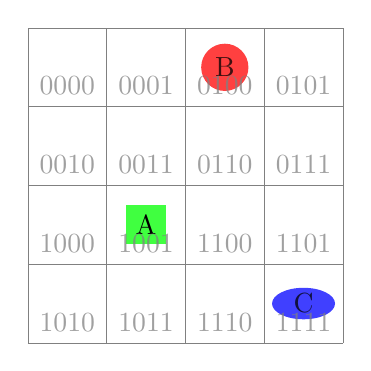
\begin{tikzpicture}
    \def\codes{{"0000","0001","0100","0101",
                "0010","0011","0110","0111",
                "1000","1001","1100","1101",
                "1010","1011","1110","1111"}}
    \draw[step=1cm,gray,very thin] (0,0) grid (4,4);
      
    \fill[red,opacity=0.75] (2.5cm,3.5cm) circle (0.3cm) node[black]{B};
    \fill[green,opacity=0.75] (1.25cm,1.25cm) rectangle (1.75cm, 1.75cm);
    \draw (1.5,1.5) node[black]{A};
    \fill[blue,opacity=0.75] (3.5,0.5) ellipse (0.4cm and 0.2cm) node[black]{C};
    \foreach \x in {0,...,3}
    \foreach \y in {0,...,3}
      \draw ( \x*1cm+0.5cm, \y*1cm+0.5cm) -- (\x*1cm+0.5cm, \y*1cm+0.5cm) node[anchor=north,gray,opacity=0.75] {\pgfmathparse{ {\codes[\x + (3-\y)*4]}}\pgfmathresult };
  \end{tikzpicture}
  \qquad
  \begin{forest}
	for tree={
	  parent anchor=south, 
	  child anchor=north,
	  align=center,
	  base=bottom
	},
	where n children=0{tier=word}{}
	[ 
          [B\\0100]
          [1
              [A\\1001] 
              [C\\1111] ] ]
  \end{forest}
  \qquad
  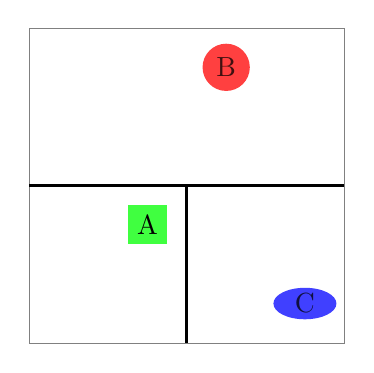
\begin{tikzpicture}
    \draw[gray,very thin] (0,0) rectangle (4,4);
    \draw[black, very thick] (0,2) -- (4,2);
    \draw[black, very thick] (2,0) -- (2,2) ;   
    \fill[red,opacity=0.75] (2.5cm,3.5cm) circle (0.3cm) node[black]{B};
    \fill[green,opacity=0.75] (1.25cm,1.25cm) rectangle (1.75cm, 1.75cm);
    \draw (1.5,1.5) node[black]{A};
    \fill[blue,opacity=0.75] (3.5,0.5) ellipse (0.4cm and 0.2cm) node[black]{C};
  \end{tikzpicture}
  \caption{Steps of constructing a kd-tree as described in \cite{Karras:2012:MPC:2383795.2383801}\\1) Assign a Morton code to each object. \\2) Sort objects and insert into binary radix tree\\3) Construct kd-tree.}
  \label{fig:tree-construction}
\end{figure}

The sorting step can be done parallelized by using some parallel sorting technique like the one introduced in \cite{Merrill:2010:RSG:1854273.1854344}.

\subsection{Traversal}
Once we have constructed an acceleration structure we need to find an efficient way to traverse it and find the closest intersection with a ray. For this report I will focus on traversing kd-trees, since "[they are] the best general purpose acceleration structure for CPU raytracers" \cite{Foley:2005} and a kd-tree is one of the outputs of the algorithm described in the previous section.
The classical traversal algorithm requires a stack to store nodes which still need to be processed. Due to the high number of rays which are processed in parallel on the GPU, a stack per ray is not feasible. This is why stackless traversal algorithms are necessary for efficient GPU ray tracing. One such algorithm is introduced by \citet{popov2007stackless}. They not only describe a technique which can travers any kd-tree without needing a stack, but also propose an efficient memory layout, taking the peculiarities of modern GPUs into consideration. A usual limitation of stackless traversal algorithm is the need to "restart" a traversal when a leaf is reached, since we cannot store which internal nodes to travers next.

\citet{popov2007stackless} get around this by storing additional information, so called "ropes", in each leaf. Ropes are pointers to the spatially adjacent nodes of a leaf. Once a leaf is reached during regular traversal we can move to the next node by following the appropriate rope based on the ray direction. This reduces the time spent on "re-traversing" the tree immensely. They also propose an efficient post-processing algorithm to add ropes to any kd-tree.

\begin{figure}[htb!]
  \centering
  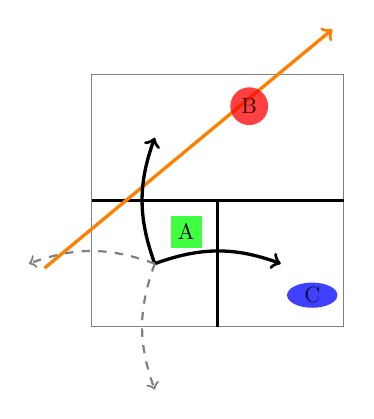
\begin{tikzpicture}[thick,scale=0.8, every node/.style={scale=0.8}]
    \draw[gray,very thin] (0,0) rectangle (4,4);
    \draw[black, very thick] (0,2) -- (4,2);
    \draw[black, very thick] (2,0) -- (2,2);   
    \draw[very thick,orange,->] (-0.75, 0.93) -- (3.82, 4.72);
    \draw[very thick,black,->] (1,1) to[bend left=20] (1,3);
    \draw[very thick,black,->] (1,1) to[bend left=20] (3,1);
    \draw[thick,dashed,gray,->] (1,1) to[bend right=20] (1,-1);
    \draw[thick,dashed,gray,->] (1,1) to[bend right=20] (-1,1);
    \fill[red,opacity=0.75] (2.5cm,3.5cm) circle (0.3cm) node[black]{B};
    \fill[green,opacity=0.75] (1.25cm,1.25cm) rectangle (1.75cm, 1.75cm);
    \draw (1.5,1.5) node[black]{A};
    \fill[blue,opacity=0.75] (3.5,0.5) ellipse (0.4cm and 0.2cm) node[black]{C};
  \end{tikzpicture}
  \qquad
  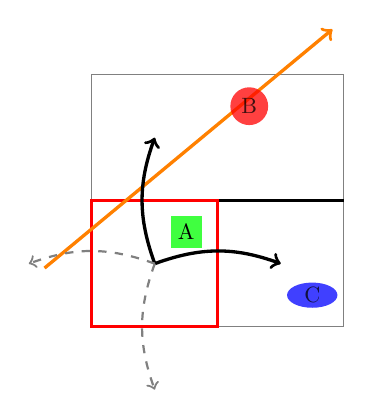
\begin{tikzpicture}[thick,scale=0.8, every node/.style={scale=0.8}]
    \draw[gray,very thin] (0,0) rectangle (4,4);
    \draw[black, very thick] (0,2) -- (4,2);
    \draw[black, very thick] (2,0) -- (2,2);  
    \draw[red,very thick] (0,0) rectangle (2,2);
    \draw[very thick,orange,->] (-0.75, 0.93) -- (3.82, 4.72);
    \draw[very thick,black,->] (1,1) to[bend left=20] (1,3);
    \draw[very thick,black,->] (1,1) to[bend left=20] (3,1);
    \draw[thick,dashed,gray,->] (1,1) to[bend right=20] (1,-1);
    \draw[thick,dashed,gray,->] (1,1) to[bend right=20] (-1,1);
    \fill[red,opacity=0.75] (2.5cm,3.5cm) circle (0.3cm) node[black]{B};
    \fill[green,opacity=0.75] (1.25cm,1.25cm) rectangle (1.75cm, 1.75cm);
    \draw (1.5,1.5) node[black]{A};
    \fill[blue,opacity=0.75] (3.5,0.5) ellipse (0.4cm and 0.2cm) node[black]{C};
  \end{tikzpicture}
  \qquad
  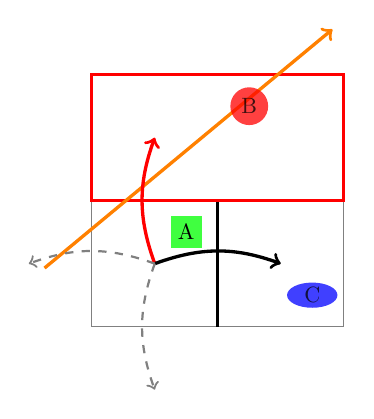
\begin{tikzpicture}[thick,scale=0.8, every node/.style={scale=0.8}]
    \draw[gray,very thin] (0,0) rectangle (4,4);
    \draw[black, very thick] (0,2) -- (4,2);
    \draw[black, very thick] (2,0) -- (2,2);  
    \draw[red,very thick] (0,2) rectangle (4,4);
    \draw[very thick,orange,->] (-0.75, 0.93) -- (3.82, 4.72);
    \draw[very thick,red,->] (1,1) to[bend left=20] (1,3);
    \draw[very thick,black,->] (1,1) to[bend left=20] (3,1);
    \draw[thick,dashed,gray,->] (1,1) to[bend right=20] (1,-1);
    \draw[thick,dashed,gray,->] (1,1) to[bend right=20] (-1,1);
    \fill[red,opacity=0.75] (2.5cm,3.5cm) circle (0.3cm) node[black]{B};
    \fill[green,opacity=0.75] (1.25cm,1.25cm) rectangle (1.75cm, 1.75cm);
    \draw (1.5,1.5) node[black]{A};
    \fill[blue,opacity=0.75] (3.5,0.5) ellipse (0.4cm and 0.2cm) node[black]{C};
  \end{tikzpicture}
  \caption{Traversing a kd-tree with ropes as proposed by \citet{popov2007stackless}. The first leaf is found as usual, afterwards we follow a rope in the appropriate direction instead of moving back up the tree.}
  \label{fig:tree-traversal}
\end{figure}


\section{Results} \label{results}
To familiarize myself with the techniques I describe in this paper I implemented a real time path tracer using C++ and OpenGL. The source code can be found at https://github.com/bonus2113/pro-se-cg.
Much of the code is based on the edge-of-space engine \cite{edge_of_space} which was built for the game programming module at RWTH Aachen in WS 15/16.
The main features are:
\begin{itemize}
\item Real time rendering of triangle models using path tracing.
\item An interactive camera system.
\item Shader hot reloading for fast iteration times.
\item TODO: FINISH FEATURE LIST
\end{itemize}

\subsection{Images}
Pretty images rendered in real time. Link to a video.
\subsection{Timings}
Timing comparisons between the different techniques.

\begin{figure}[htb!]
  \begin{centering}
    \includegraphics[width=10cm,natwidth=1920,natheight=1080]{figures/Output_PT_10kSPP.png}\par
  \end{centering}
  \caption{This is what my path tracer is rendering right now, but not in real time.}
  \label{fig:pathtraced}
\end{figure}

%%%%%%%%%%%%%%%%%%%%%%%%%%%%%%%%%%%%%%%%%%%%%%%%%%%%%%%%%%%%
% Bibliography

\printbibliography


\end{document}
